\chapter{基于内存压力的自动卸载框架}
\label{chap:基于内存压力的自动卸载框架}
在\ref{chap:基于同步内存回收的内存压力量化算法的设计与实现}中,已将同步内存回收量化为内存压力。基于量化的压力值,用户态的内存压力感知卸载框架可以主动将冷页面卸载到异构后端。本章将介绍基于proc文件系统的mpfs实现、基于内存压力的工作集估计算法以及基于访问距离的匿名页和文件页的平衡算法。


\section{内存压力文件系统的实现}
\label{sec:mpfs_implementation}

基于\ref{sec:基于同步回收延迟的内存压力量化实现}章节实现的内存压力量化模型,本节构建用户态调控接口以实现冷页面的动态卸载机制。选择用户态实现方案可有效提升策略迭代效率,同时支持基于 QoS 需求的差异化策略配置。

\subsection{proc 文件系统架构分析}

proc 文件系统作为内核与用户态间的标准交互接口,其设计具有以下核心特征:

\begin{itemize}
    \item \textbf{动态生成机制:} 文件节点根据内核运行时状态实时构建
    \item \textbf{虚拟存储特性:} 不占用物理存储空间,通过内存映射实现数据存取
    \item \textbf{双向交互能力:} 支持通过标准I/O系统调用进行内核参数查询与配置
    \item \textbf{抽象访问层:} 对用户态程序隐藏内核数据结构复杂性,提供统一访问范式
\end{itemize}

上述特性使其成为实现跨态内存压力交互的理想媒介。

\subsection{mpfs 系统架构设计}

本系统通过设计内存压力文件系统(Memory Pressure File System, mpfs)实现以下核心功能:

\begin{itemize}
    \item \texttt{/proc/mpfs/mem\_pressure}:提供实时内存压力值轮询接口,支持事件驱动通知机制
    \item \texttt{/proc/mpfs/period}:实现采样周期动态可配置接口(时间单位:秒)
    \item \texttt{/proc/mpfs/mthreshold}:设置压力阈值触发条件(百分比形式)
\end{itemize}

表 \ref{tab:mpfs_files} 详细描述了各文件接口的操作语义及功能映射关系。

\begin{table}[H]
    \centering
    \caption{mpfs 文件系统接口规范}
    \label{tab:mpfs_files}
    \begin{tabular}{lccc}
        \toprule
        \textbf{操作类型} & \texttt{mem\_pressure} & \texttt{period} & \texttt{mthreshold} \\
        \midrule
        \texttt{read} & 读取当前压力值 & 获取采样周期 & 查询当前阈值 \\
        \texttt{write} & - & 更新采样周期 & 修改触发阈值 \\
        \texttt{poll} & 事件通知机制 & - & - \\
        \bottomrule
    \end{tabular}
\end{table}

\subsection{内核模块实现细节}

系统通过注册内核模块实现功能组件,核心流程如下:

\begin{itemize}
    \item \textbf{模块初始化:} 通过 \texttt{proc\_create} 在 \texttt{/proc/mpfs} 目录下创建三个虚拟文件节点,分别绑定对应的文件操作函数集(\texttt{file\_operations})
  
    \item \textbf{压力值读取:}
    \begin{itemize}
        \item \texttt{mempressure\_read} 函数从原子变量 \texttt{current\_usage\_percent} 获取压力值
        \item 采用 \texttt{sprintf} 格式化输出保证数据可读性
    \end{itemize}

    \item \textbf{事件通知机制:}
    \begin{itemize}
        \item \texttt{mempressure\_poll} 将进程加入等待队列 \texttt{mem\_waitq}
        \item 当工作队列计算出压力值后,如果超出了阈值,将唤醒等待队列 \texttt{mem\_waitq} 上的所有进程
        \item 当 \texttt{pressure\_flag} 置位时返回 \texttt{POLLIN | POLLRDNORM} 状态码
    \end{itemize}

    \item \textbf{参数动态配置:}
    \begin{itemize}
        \item 采样周期更新函数 \texttt{mempressure\_period\_write} 包含整型参数校验逻辑
        \item 阈值修改函数 \texttt{mempressure\_threshold\_write} 实施百分比有效性验证
    \end{itemize}
\end{itemize}

该架构通过标准文件接口实现用户态策略与控制参数的动态注入,同时保证内核态监测机制的实时响应能力。



\section{基于内存压力的动态调控模型}
\label{sec:pressure_based_model}

传统工作集估计方法依赖内核态时间、应用吞吐量变化率、回收事件计数器等间接指标,其有效性受限于运维人员对存储硬件特性与内核行为的专业认知。在\ref{chap:基于同步内存回收的内存压力量化算法的设计与实现}中,本研究提出基于同步内存回收的压力指标,可以自适应不同的负载和异构卸载后端。本节我们就基于定义的内存压力,来实现基于内存压力的动态调控。此模型采用主动回收策略,通过监控系统内存压力来维持目标压力区间,并将低访问频率数据页迁移至基于`frontswap`的异构存储后端,从而实现内存利用率的优化。

\begin{figure}[h]
\centering
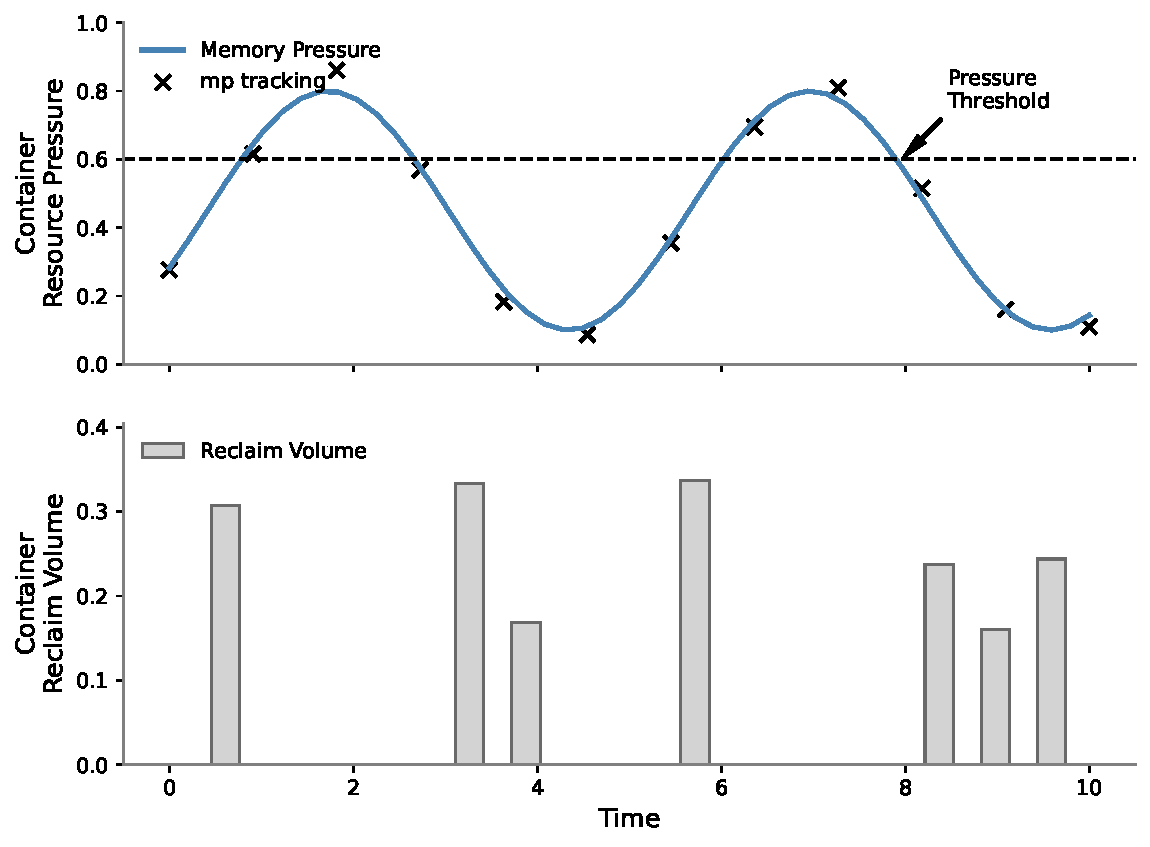
\includegraphics[width=0.95\textwidth]{压力与回收.pdf}
\caption{内存压力与页面回收调控机制}
\label{fig:pressure_work_set}
\end{figure}

本算法通过压力量化与反馈机制来实现内存的动态调控。不同于传统的静态内存管理策略,本算法根据系统的实时内存压力调整内存的使用范围,确保系统在高负载时能够扩展内存资源,在低负载时又能将冷页面主动卸载。这种基于内存压力的调控方法能够有效应对突发负载变化,并在保证系统稳定性的同时,提高内存资源的利用率。

图\ref{fig:pressure_work_set}展示了本模型的设计目标,即通过监控系统的内存压力,采用动态调整策略,确保系统内存处于合理的使用范围内。具体而言,当系统内存压力超过设定目标时,系统会逐步放宽内存限制;反之,内存压力较低时,系统会收紧内存限制。这样,不仅能在高负载时避免内存不足的问题,还能在低负载时将冷页面主动卸载。

本算法采用压力积分反馈机制,其中的关键参数体系如表\ref{tab:params}所示。算法每6秒钟执行一次,设定一个目标内存压力阈值,实现系统的平滑调节。累积的压力误差是通过比较实际内存压力与目标内存压力阈值的差异来计算的,从而形成一个时间窗口内的压力累积效应。



\begin{table}[H]
\centering
\caption{调控参数体系}
\label{tab:params}
\begin{tabular}{cccc}
\toprule
参数 & 符号 & 默认值 & 作用域 \\
\midrule
目标压力 & \(mem\_pressure\_target\) & 0.1\% & 全局 \\
最大收缩率 & \(M_p\) & 0.01 & 缩容阶段 \\
最大扩张率 & \(M_b\) & 1.0 & 扩容阶段 \\
收缩灵敏度 & \(C_p\) & 10 & 缩容触发 \\
扩张灵敏度 & \(C_b\) & 20 & 扩容触发 \\
\bottomrule
\end{tabular}
\end{table}

\begin{algorithm}[H]
    \caption{基于压力的内存调控算法}
    \label{alg:control}
    \Input{\(mem\_pressure\), \(mem\_pressure\_target\), \(C_b\), \(C_p\), \(M_b\), \(M_p\), \(min\_size\), \(max\_size\)}
    \Output{Memory Limit \(Limit\)}
    \While{\textrm{true}}{  
        \(mem\_pressure\) get from proc file system;\\
        \If{\(mem\_pressure > mem\_pressure\_target\)}{
            % Calculate expansion coefficient eta
            \(\eta \leftarrow \min\left(\left(\frac{mem\_pressure/mem\_pressure\_target}{C_b}\right)^2, 1\right)\)*\(M_b\)\;
            % Perform expansion
            \(Limit \leftarrow \min(max\_size, Limit \times (1 + \eta))\)\;
            }
        \Else{
            % Calculate contraction coefficient eta
            \(\eta \leftarrow \min\left(\left(\frac{mem\_pressure\_target/mem\_pressure}{C_p}\right)^2, 1\right)\)*\(M_p\)\;
            % Perform contraction
            \(Limit \leftarrow \max(min\_size, Limit \times (1 - \eta))\)\;
            }
        % Apply the new memory limit
        Apply new memory limit \(Limit\)\;
    }
\end{algorithm}

\begin{itemize}
\item \textbf{灵敏度系数(\(C_p, C_b\))}: 
  \begin{itemize}
  \item 扩张灵敏度\(C_b=20\): 当累积压力超过目标值20倍时达到最大扩容比例
  \item 收缩灵敏度\(C_p=10\): 当压力低于目标值1/10时触发最大缩容
  \end{itemize}

\item \textbf{最大比例(\(M_p, M_b\))}: 
  \begin{itemize}
  \item \(M_b=1.0\)允许单次扩容100\%,应对突发压力
  \item \(M_p=0.01\)限制单次缩容1\%,确保服务稳定性
  \end{itemize}

\item \textbf{积分机制}: 
  \begin{itemize}
  \item 累积窗口\(T_{interval}=6s\)平滑瞬时波动
  \item 压力增量\(\Delta P\)累计检测持续负载
  \end{itemize}
\end{itemize}

本算法的设计考虑了内存压力的动态变化与不同负载场景下的需求,因此参数体系中包含了多种灵敏度、最大收缩比例、扩张比例等调控因子,用于灵活应对系统的负载变化。例如,扩张灵敏度\(C_b = 20\)表示当实际内存压力超过目标压力的20倍时,系统会达到最大扩容比例;收缩灵敏度\(C_p = 10\)则表示当实际内存压力低于目标压力的1/10时,系统会触发最大缩容。

最大扩张比例\(M_b = 1.0\)允许单次扩容至最大限制的100\%,应对突发的内存压力;而最大收缩比例\(M_p = 0.01\)限制单次缩容不超过1\%,确保系统的稳定性,避免因过快的收缩而导致服务质量下降。通过这些参数的调整,系统能够灵活应对不同的负载条件,避免内存资源的过度浪费,并确保在需要时能够快速扩展内存。


需要特别强调的是,上述算法只是一个示例,目的是展示如何基于内存压力进行动态调控。在实际应用中,用户可以根据不同的服务质量(QoS)要求、系统负载特性或硬件架构,单独配置这些参数,甚至根据负载类型重新定义内存调控策略。例如,在某些高实时性应用中,可能会选择较高的扩张灵敏度 \(C_b\) 和较低的收缩灵敏度 \(C_p\),以确保快速响应压力变化。而在对于一般后台任务的处理上,则可能会选用较为保守的策略,以确保稳定性和节省资源。

通过采用灵活配置的方式,本算法能够根据不同的需求调整内存压力阈值、调节因子和策略参数,从而提供更具针对性和适应性的内存管理策略。算法的灵活性使得它能够适用于不同的负载场景和硬件环境,满足各种不同应用的内存管理需求。

此外,该算法可以结合不同的内存管理机制,如基于事件驱动的非阻塞方法,避免轮询带来的性能损失。未来也可以通过引入机器学习或预测算法,自动调整调控策略和参数,以实现更加智能和自适应的内存管理。算法本身也可以与其他资源管理策略结合,共同优化系统的整体性能和资源分配。
、
% \section{内存压力文件系统的实现}
% \label{sec:mpfs_implementation}

% 在\ref{sec:基于同步回收延迟的内存压力量化实现}中,本研究已经实现了基于同步回收延迟的内存压力量化实现,我们需要根据压力来进行调控,实现冷页面的自动卸载。在用户态实现可以更快进行迭代,也可以根据负载的实际的QOS来设置不同的策略。

% 所以本研究需要将压力的值暴露给用户态,通过proc文件系统来实现是一个很好的方法。

% \subsubsection{proc 文件系统概述}

% proc 文件系统是一种特殊的、由内核动态生成的伪文件系统,通常挂载于 /proc 目录。它并不存储在物理磁盘上,而是存在于内存中,为用户空间提供了一种访问和修改内核信息的标准接口。proc 文件系统具有以下几个关键特性:

% \begin{itemize}
%     \item \textbf{动态性:} proc 文件系统中的文件和目录并非静态存在,而是由内核根据当前系统状态动态生成。
%     \item \textbf{虚拟性:} proc 文件系统中的文件不占用实际的磁盘空间,它们只是内核数据的虚拟表示。
%     \item \textbf{交互性:} 用户可以通过标准的文件 I/O 操作(如 \texttt{read}、\texttt{write}、\texttt{poll} 等)与 proc 文件系统中的文件进行交互,从而读取内核信息或修改内核参数。
%     \item \textbf{通用性:} proc 文件系统提供了一套统一的接口,使得用户空间的应用程序无需了解内核内部的复杂数据结构,即可方便地访问内核信息。
% \end{itemize}

% 基于 proc 文件系统的这些特性,它非常适合作为用户态与内核态之间进行信息交换的桥梁。

% \subsubsection{mpfs 的设计与实现}

% \texttt{mpfs} 的设计目标是提供一个轻量级、响应及时的接口,供用户态程序获取和监控系统的内存压力信息,并支持基于内存压力的事件通知机制。为了实现这一目标,\texttt{mpfs} 提供了以下三个文件接口:

% \begin{itemize}
%     \item \texttt{/proc/mpfs/mem\_pressure}:用于读取当前系统的内存压力值(百分比)。该文件支持 poll 系统调用,当内存压力超过预设阈值时,会触发可读事件,从而通知等待中的用户态程序。
%     \item \texttt{/proc/mpfs/period}:用于读取和设置内存压力采样周期(单位:秒)。用户态程序可以通过写入该文件来动态调整采样频率。
%     \item \texttt{/proc/mpfs/mthreshold}:用于读取和设置内存压力阈值(百分比)。当内存压力超过该阈值时,\texttt{/proc/mpfs/mem\_pressure} 文件的 poll 调用会返回可读事件。
% \end{itemize}

% 表 \ref{tab:mpfs_files} 总结了 mpfs 中各个文件接口及其对应的文件操作函数。

% \begin{table}[H]
%     \centering
%     \caption{mpfs 文件接口及操作}
%     \label{tab:mpfs_files}
%     \begin{tabular}{cccc} % 四列,都居中对齐
%         \toprule
%         \textbf{操作} & \textbf{\texttt{/proc/mpfs/mem\_pressure}} & \textbf{\texttt{/proc/mpfs/period}} & \textbf{\texttt{/proc/mpfs/mthreshold}} \\
%         \midrule
%         \texttt{read} & 获取内存压力 & 获取采样周期 & 获取压力阈值 \\
%         \texttt{write} &  & 设置采样周期 & 设置压力阈值 \\
%         \texttt{poll} & 内存压力事件通知 &  &  \\
%         \bottomrule
%     \end{tabular}
% \end{table}


% mpfs 的核心实现基于内核模块机制。在模块初始化函数 (mempressure\_init) 中,通过 proc\_create 函数创建了上述三个文件节点,并分别指定了它们的文件操作函数集(file\_operations 结构)。

% \begin{itemize}
%     \item \textbf{\texttt{mem\_pressure}} 文件:
%     \begin{itemize}
%         \item \texttt{read} 操作:调用 \texttt{mempressure\_read} 函数,从全局静态变量处获取当前内存压力值,并将其格式化为字符串后复制到用户空间缓冲区。
%         \item \texttt{poll} 操作:调用 \texttt{mempressure\_poll} 函数,该函数首先将当前进程添加到等待队列 \texttt{mem\_waitq} 中,然后调用\texttt{mempressure\_read}查看内存压力,。如果内存压力超过阈值,则返回 \texttt{POLLIN | POLLRDNORM},表示文件可读;否则,进程将进入睡眠状态,等待被唤醒。
%     \end{itemize}

% \item \textbf{\texttt{period}} 文件:
%     \begin{itemize}
%         \item \texttt{read} 操作:调用 \texttt{mempressure\_period\_read} 函数,该函数读取全局变量 \texttt{sample\_period}(采样周期,单位:秒),并将其格式化为字符串后复制到用户空间缓冲区。
%         \item \texttt{write} 操作:调用 \texttt{mempressure\_period\_write} 函数,该函数从用户空间缓冲区读取新的采样周期值,并进行合法性检查(必须为正整数)。然后更新采样周期,等到之后工作队列就可以采用新的采样周期。
%     \end{itemize}

%     \item \textbf{\texttt{mthreshold}} 文件:
%     \begin{itemize}
%     \item \texttt{read} 操作:调用 \texttt{mempressure\_threshold\_read} 函数,该函数读取全局变量 \texttt{mem\_pressure\_threshold}(内存压力阈值,百分比),并将其格式化为字符串后复制到用户空间缓冲区。
%     \item \texttt{write} 操作:调用 \texttt{mempressure\_threshold\_write} 函数,该函数从用户空间缓冲区读取新的阈值,并进行合法性检查)。然后更新阈值就可以返回。
%     \end{itemize}
% \end{itemize}

% 内存压力的周期性监测和事件通知由工作队列 \texttt{pressure\_work} 实现。工作队列的处理函数 \texttt{mempressure\_workfunc} 执行以下操作:

% \begin{enumerate}
%     \item 获取系统内存信息(总内存、可用内存),计算内存使用率(百分比)。
%     \item 将计算得到的内存使用率更新到原子变量 current\_usage\_percent。
%     \item 检查内存使用率是否超过阈值 mem\_pressure\_threshold。如果超过,则设置内存压力标志 pressure\_flag,并通过 wake\_up\_interruptible 函数唤醒等待队列 mem\_waitq 上的所有进程。
%     \item 根据当前采样周期 sample\_period 重新调度工作队列 pressure\_work。
% \end{enumerate}

% 通过上述设计和实现,mpfs 为用户态程序提供了一个简洁、高效的接口,用于实时监控系统内存压力,并根据需要调整采样周期和阈值。



\section{基于重用距离的冷热页面优化}
\label{sec:基于重用距离的冷热页面优化}


% \subsection{重用距离}

% 受到文献\cite{jiang2002lirs,jiang2005clockpro}关于重用距离(Reuse Distance)研究的启发,我们尝试引入重用距离这一概念来平衡文件页面与匿名页面的回收策略。重用距离刻画了某个页面两次访问之间,被访问过的不同页面的数量,能从更广阔的角度度量页面的使用频率及其在内存替换时的优先级。

% 对一段内存访问序列
% \[
%     A = \{a_1,\, a_2,\, a_3,\dots,a_n\},
% \]
% 令 \(a_i\) 表示第 \(i\) 次访问的页面编号。页面 \(P\) 的重用距离可定义为
% \begin{equation}
%   \label{eq:rd_def}
%   RD(P) \;=\; \min \bigl\{\, j - i \,\bigm|\,
%   a_i = P,\; a_j = P,\; i < j \bigr\},
% \end{equation}
% 即在页面 \(P\) 第一次被访问(索引 \(i\))到第二次被访问(索引 \(j\))之间,出现的不同页面数的最小可能值。若某页面的重用距离很短,则意味着其访问非常频繁;若重用距离较长,则该页面在替换算法中往往是更好的回收对象。

% \begin{figure}[htbp]
%   \centering
%   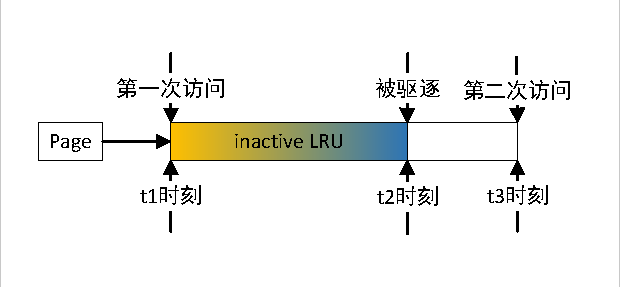
\includegraphics[width=0.5\textwidth]{重用距离.pdf}
%   \caption{重用距离示意图}
%   \label{fig:refault_distance}
% \end{figure}

% 然而,在实践中逐页追踪重用距离往往需要为每一页维护完整的历史访问信息,这在大型系统中会带来可观的存储和维护成本。为了降低开销,我们采用近似方法:观察页面在活动链表(Active List)和非活动链表(Inactive List)之间的迁移,以推断其访问频度;当页面重新被访问时,若该页面曾被替换出去(即从非活动链表被驱逐),则说明在它被驱逐至再次访问的这段时间里,系统至少经历了一定数量的页面访问。

% \subsection{重用距离的近似推导}

% 为了直观地分析非活动链表上的页面行为,我们做如下简化假设:非活动链表长度固定,且暂不考虑活动链表中的页面降级至非活动链表的情形。这样可更专注于分析非活动链表本身的访问与替换规律。在此前提下,图 \ref{fig:现象1} 与图 \ref{fig:现象2} 展示了两种典型场景:

% \begin{figure}[htbp]
%   \centering
%   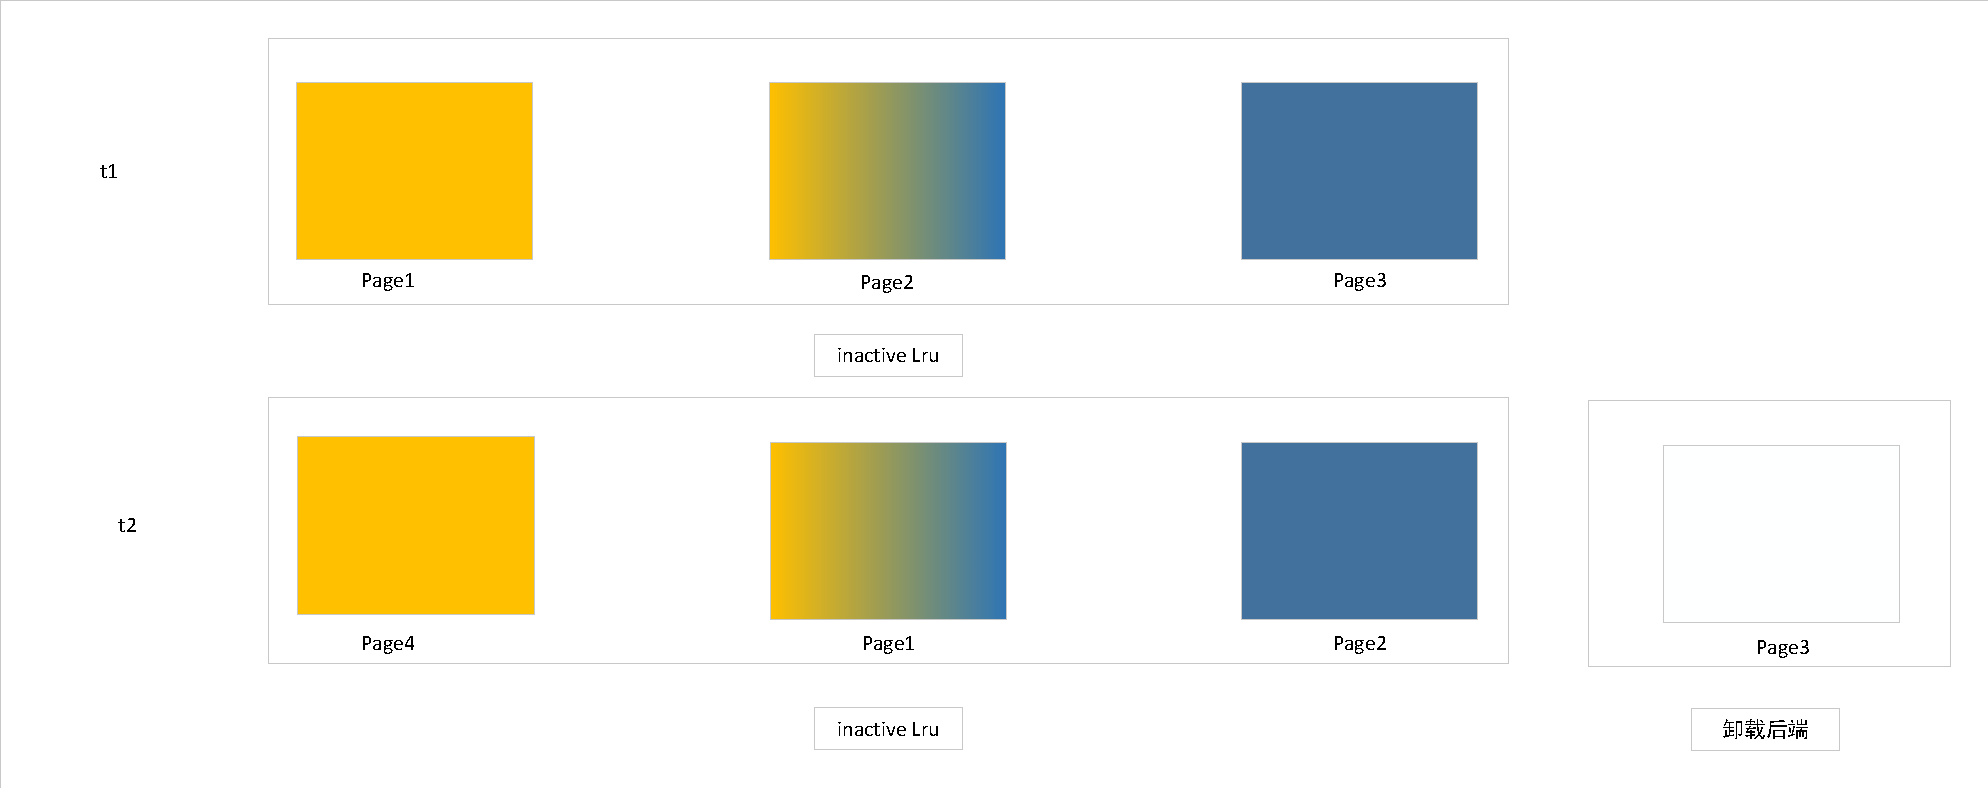
\includegraphics[width=0.5\textwidth]{现象1.pdf}
%   \caption{情形一:页面首次插入非活动链表}
%   \label{fig:现象1}
% \end{figure}

% \begin{figure}[htbp]
%   \centering
%   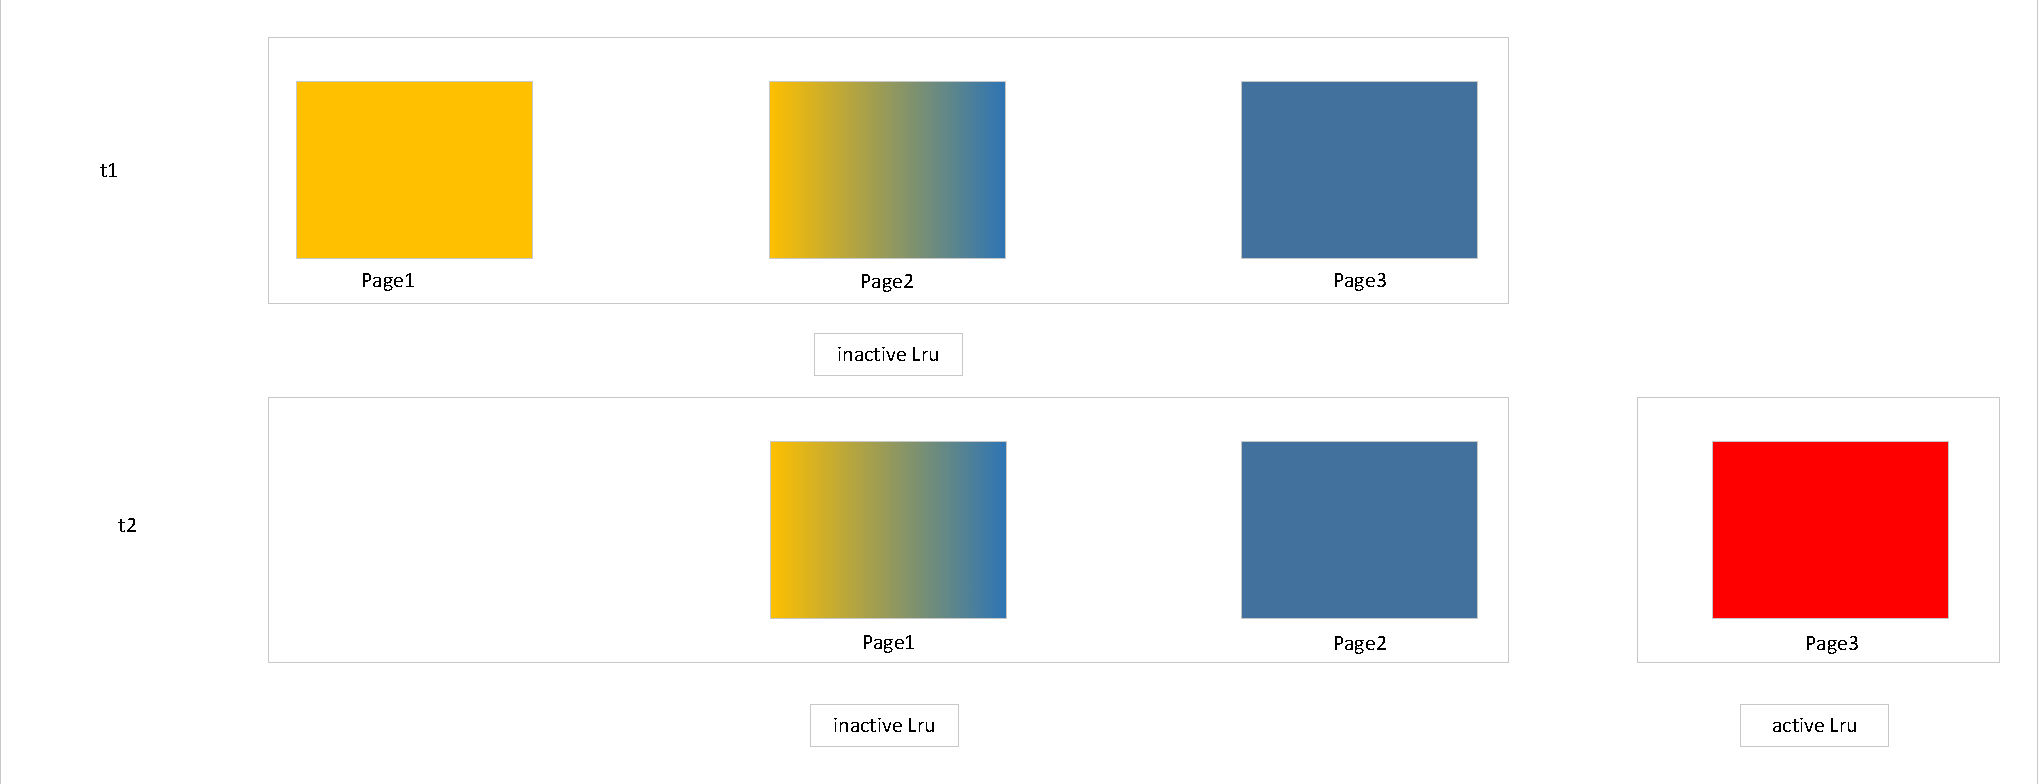
\includegraphics[width=0.5\textwidth]{现象2.pdf}
%   \caption{情形二:页面在非活动链表上再次被访问并提升到活动链表}
%   \label{fig:现象2}
% \end{figure}
% \begin{itemize}
%   \item 情形一(图 \ref{fig:现象1})对应页面第一次访问并被插入到非活动链表头部。由于非活动链表长度固定,原先在链表中的页面会整体向尾部滑动,最终导致最末尾的页面被挤出内存(即被驱逐)。  
%   \item 情形二(图 \ref{fig:现象2})对应页面在非活动链表上再次被访问并提升到活动链表,这同样会使非活动链表缩短一个位置,同时,所有比被提升页面更晚载入非活动链表的页面都会被推向尾部,从而离被驱逐更近。
% \end{itemize}

% 基于这两种主要行为,可以观察到:在时间区间 \([t_1, t_2]\) 内,非活动链表的页面要么被驱逐(表明一定有新页面加载)、要么被提升至活动链表(表明其被再次访问)。令
% \(
%   E(t_1,t_2)
% \)
% 表示在 \([t_1,t_2]\) 区间内的驱逐次数(evictions),令
% \(
%   A(t_1,t_2)
% \)
% 表示在该区间的页面提升次数(activations)。由于每次驱逐意味着至少加载了一个新的页面,每次提升代表至少发生了一次对非活动链表中页面的访问,故可以近似认为,在 \([t_1,t_2]\) 时间段里,系统产生的最少页面访问数不低于
% \begin{equation}
%   E(t_1,t_2) \;+\; A(t_1,t_2).
% \end{equation}
% 在实际系统中,尚需考虑其他潜在行为,例如“始终位于活动链表且未被降级的页面访问数”。不过,对于那些访问特别频繁的页面,因其始终活跃,我们往往无需担心它们被回收或缺少统计;换言之,这部分页面对近似分析的影响有限,而我们更需要关注的是可能进入或留在非活动链表的页面。



% % \paragraph{重新故障距离 的定义与计算}

% 当一个页面 \(p\) 被驱逐时,我们在驱逐时刻 \(t_1\) 记录一个计数器值 \({count}(t_1)\),它反映的是系统自启动至 \(t_1\) 时刻所累计的“驱逐次数 + 提升次数”(即 \(E + A\))。一旦该页面在时刻 \(t_2\) 再次被访问,我们同样记录 \({count}(t_2)\)。基于前述分析,可定义页面 \(p\) 的重新故障距离(Refault Distance)为
% \begin{equation}
%   \label{eq:refault_distance}
%   D_{\mathrm{refault}}(p)
%   \;=\;
%   \mathrm{count}(t_2)
%   \;-\;
%   \mathrm{count}(t_1),
% \end{equation}
% 它衡量了页面在被驱逐后到再次访问期间,系统所经历的最少页面访问数量。

% 若我们进一步近似页面在内存中的时候访问的页面数量使用非活动链表中的位置数 \(\displaystyle L_{\mathrm{inactive}}\),则可近似推断页面 \(p\) 的总“访问距离”为
% \begin{equation}
%   \label{eq:dtotal}
%   D_{\mathrm{total}}(p)
%   \;=\;
%   L_{\mathrm{inactive}}
%   \;+\;
%   \bigl(\mathrm{count}(t_2) - \mathrm{count}(t_1)\bigr).
% \end{equation}
% 其中,\(\displaystyle L_{\mathrm{inactive}}\) 是用来衡量“页面在非活动链表中一旦越往后排,就越接近被驱逐”的事实。直观来看,若非活动链表本身长度较小且页面常被迅速驱逐,那么一段时间内的 \(\mathrm{count}(\cdot)\) 增量就会变大,说明系统在该时段里确实经历了大量访问,也意味着较长的重用距离或低访问频度。

% \subsection{替换决策与回收策略}

% 结合活动链表的大小 \(\displaystyle L_{\mathrm{active}}\) 进行分析,若我们希望某页面在内存中继续保留,则需要满足
% \begin{equation}
%   \label{eq:active_condition}
%   L_{\mathrm{inactive}}
%   \;+\;
%   \bigl(\mathrm{count}(t_2) - \mathrm{count}(t_1)\bigr)
%   \;\;\le\;\;
%   L_{\mathrm{inactive}}
%   \;+\;
%   L_{\mathrm{active}},
% \end{equation}
% 即化简后 
% \[
%   \mathrm{count}(t_2) - \mathrm{count}(t_1)
%   \;\le\;
%   L_{\mathrm{active}}.
% \]
% 这说明,如果页面的重新故障距离小于或等于活动链表的容量,那么它的访问频度足以支撑其继续留驻在内存中,不应被轻易替换。

% 此外,此类基于重用距离或重新故障距离的估算,还可以与系统的 \(\mathrm{swappiness}\) 参数结合,用来调度文件页与匿名页之间的回收比例。例如:
% \[
%   \mathrm{swappiness} 
%   \;=\;
%   \min\!
%   \Bigl(
%     \mathrm{swappiness}
%     \,\times\,
%     \bigl(1 \,+\, \mathrm{refault\_active}\bigr),
%     \;150
%   \Bigr),
% \]
% 其中 \(\mathrm{refault\_active}\) 可以被视为在近期内发生的“重新故障”事件所占比重,通过该比重调整文件页和匿名页的回收策略,以在系统负载与访问模式变化时,动态地优化内存利用效率。

% 综上所述,通过上述驱逐次数与提升次数的近似推断,我们在非活动链表的页面行为上获取了低成本的访问统计依据。这样不仅免去了逐页计算完整重用距离的高开销,也能够在大多数真实场景中较准确地识别频繁访问的页面。借助这些统计,我们更容易针对文件页与匿名页制定适配性回收策略,从而在提高缓存命中率的同时,也能有效降低内存压力,从整体上优化系统性能与资源利用率。

\subsection{重用距离}

受到文献 \cite{jiang2002lirs,jiang2005clockpro} 对重用距离(Reuse Distance)的研究启发,我们将其引入页面替换策略的设计,以在文件页面与匿名页面的回收之间取得更佳平衡。重用距离刻画某一页面两次访问之间,被访问过的不同页面的数量,能在一定程度上反映页面的访问模式及其在替换时的优先级。

对一段内存访问序列
\[
  A \;=\;\{\,a_1,\,a_2,\,\dots,\,a_n\},
\]
其中 \(a_i\) 表示第 \(i\) 次访问的页面。令 \(P\) 为所关心的目标页面,则可将其重用距离定义为
\begin{align}
\label{eq:rd_def}
  RD(P) 
  &= 
  \min\Bigl\{\,j - i
    \;\Bigm|\;
    a_i = P,\;
    a_j = P,\;
    i < j
  \Bigr\}.
\end{align}
直观而言,若 \(RD(P)\) 较短,则页面 \(P\) 被访问得更为频繁;若 \(RD(P)\) 较长,则表明其访问稀疏,往往可作为回收候选。

\begin{figure}[htbp]
  \centering
  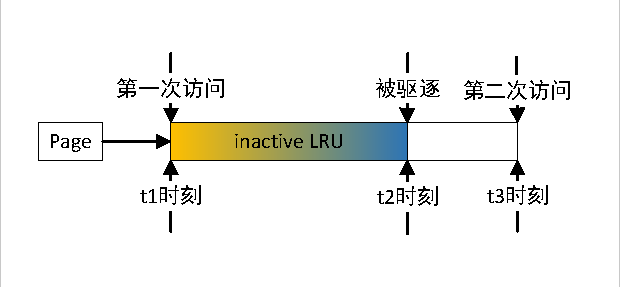
\includegraphics[width=0.5\textwidth]{重用距离.pdf}
  \caption{重用距离示意图}
  \label{fig:refault_distance}
\end{figure}

然而,在大型系统中为每个页面维护完整的访问信息以精确计算重用距离需要占用大量存储空间与数据结构维护开销。为此,我们借助近似策略:通过观察页面在活动链表(Active List)与非活动链表(Inactive List)间的迁移规律,来间接推断页面被访问的频度。当某页面在非活动链表上被替换(即被驱逐)后,若它在短期内再次被访问,即说明在此期间系统至少经历了一定数量的页面访问,从而可近似估计该页面的访问频率。


\subsection{重用距离的近似推导}

为了简化分析,先假设非活动链表长度固定,且暂不考虑活动链表向非活动链表的降级。这样可以更直观地专注于非活动链表上的页面替换与访问。图 \ref{fig:现象1} 与图 \ref{fig:现象2} 展示了两种核心场景。

\begin{figure}[htbp]
  \centering
  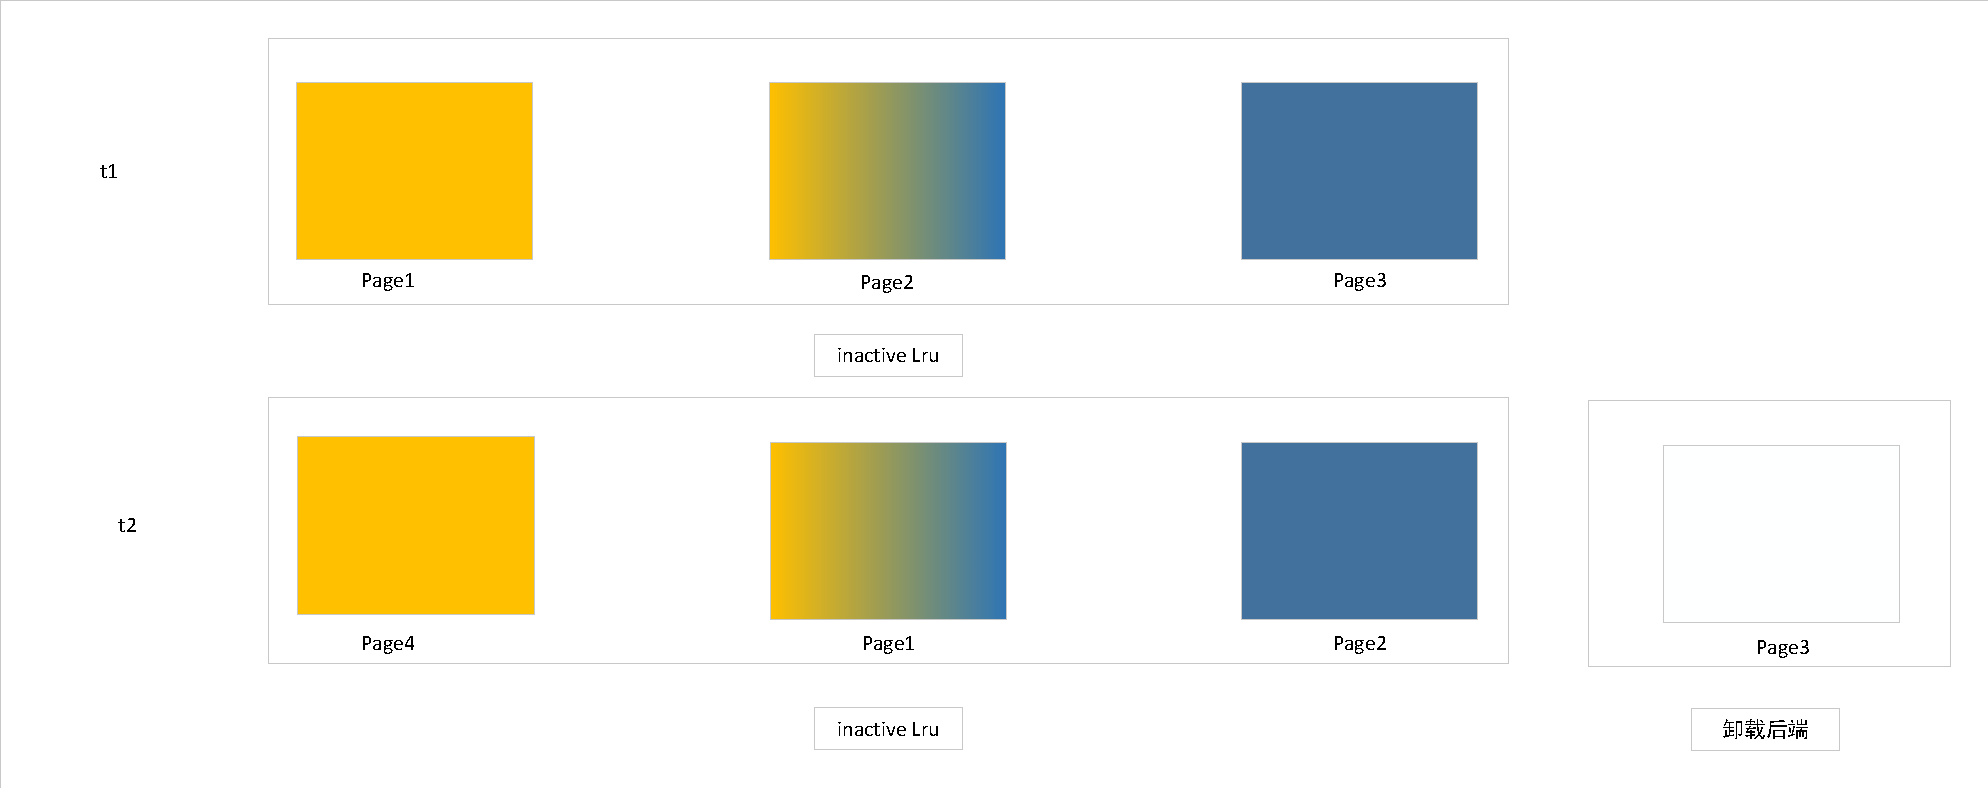
\includegraphics[width=0.5\textwidth]{现象1.pdf}
  \caption{情形一:页面首次插入非活动链表}
  \label{fig:现象1}
\end{figure}

\begin{figure}[htbp]
  \centering
  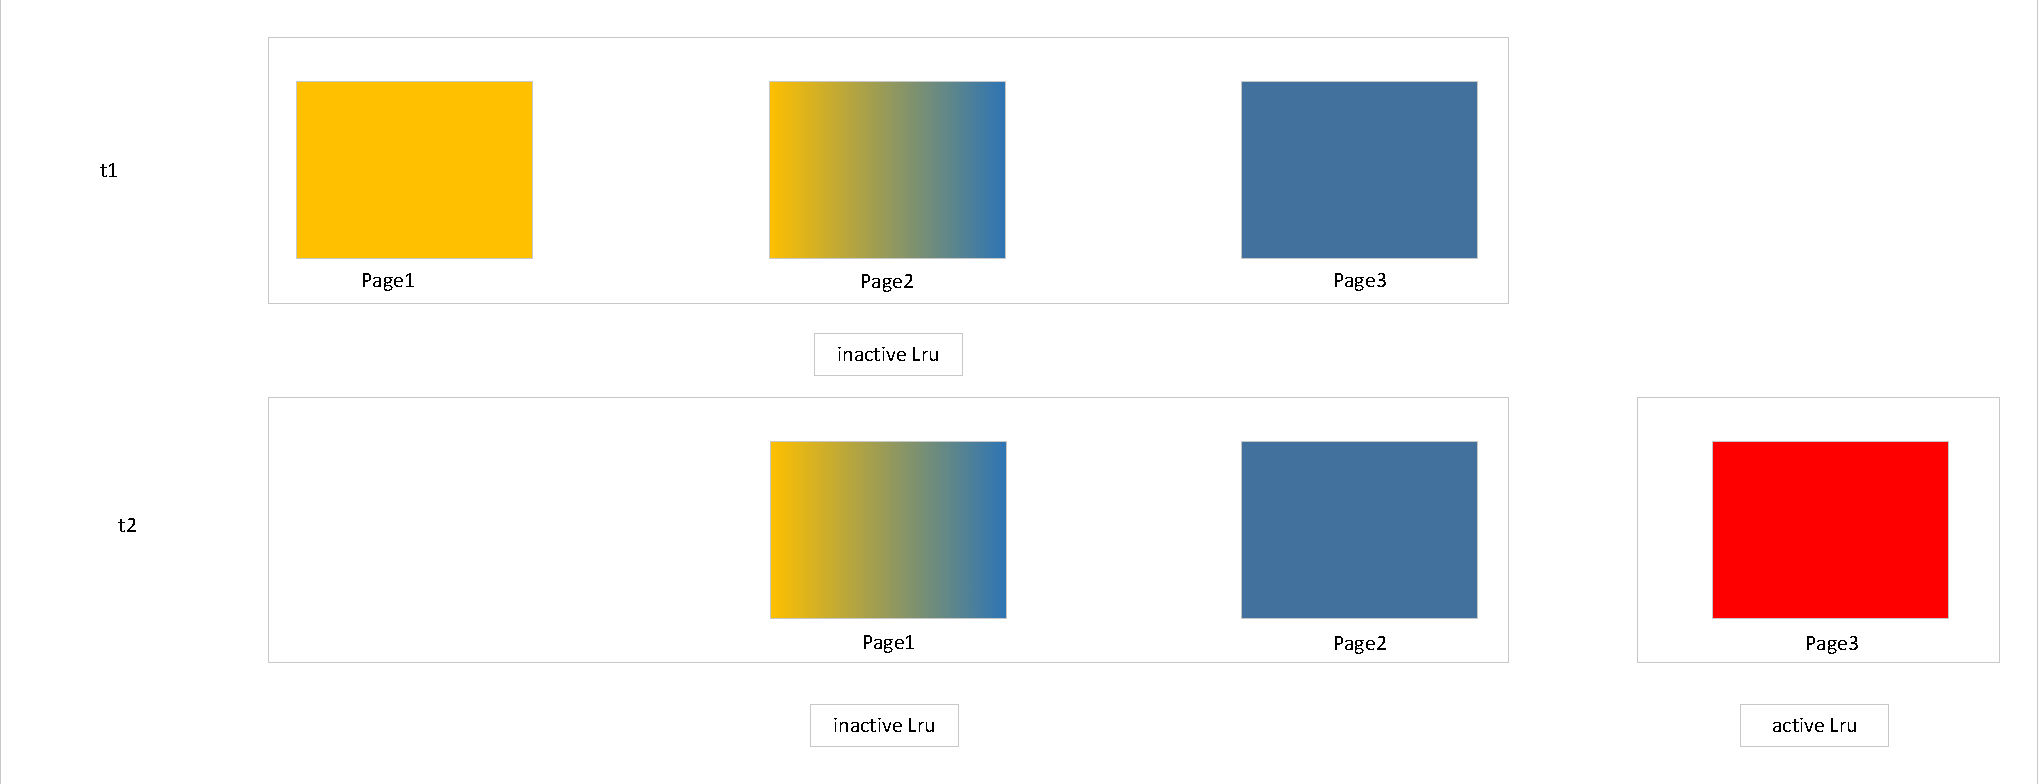
\includegraphics[width=0.5\textwidth]{现象2.pdf}
  \caption{情形二:页面在非活动链表上再次被访问并提升到活动链表}
  \label{fig:现象2}
\end{figure}

\noindent
\textbf{情形一}(图 \ref{fig:现象1})描述页面首次被访问并插入到非活动链表头部;由于链表长度固定,原链表中的页面整体向尾部滑动,最末尾页面被挤出内存(驱逐)。  
\textbf{情形二}(图 \ref{fig:现象2})描述页面在非活动链表上再次被访问后,被“提升”到活动链表,链表长度相应缩短;与此同时,所有比被提升页面更晚进入非活动链表的页面向尾部滑动,离被驱逐更近。

在时间区间 \([t_1, t_2]\) 内,非活动链表上的页面要么被驱逐(表明至少加载了新的页面),要么被提升至活动链表(表明被再次访问)。令
\[
  E(t_1,t_2)
\]
表示该区间内的驱逐次数(evictions),令
\[
  A(t_1,t_2)
\]
表示该区间的页面提升次数(activations)。因为每次驱逐对应至少一次新页面的载入,每次提升对应至少一次对非活动链表中页面的访问,故可以近似认为 \([t_1,t_2]\) 时间段内发生的最少页面访问数不低于
\begin{align}
  \label{eq:e_plus_a}
  E(t_1,t_2) \;+\; A(t_1,t_2).
\end{align}
真实系统中还需考虑一直停留在活动链表、从未降级的页面访问量。不过,对访问极频繁的页面而言,由于它们并不进入非活动链表,我们无需担心其“再次访问”情形的遗漏,因此对这部分页面的统计影响相对有限。


当页面 \(p\) 被驱逐时,我们记录其驱逐时刻 \(t_1\) 对应的计数器 \(\mathrm{count}(t_1)\),该计数器反映系统自启动至 \(t_1\) 时刻产生的驱逐次数与提升次数之和。

若该页面于时刻 \(t_2\) 再次被访问,则同样记录 \(count(t_2)\)。此时,我们定义页面 \(p\) 的重新故障距离(Refault Distance)为
\begin{align}
  \label{eq:refault_distance}
  D_{\mathrm{refault}}(p)
  &= 
  \mathrm{count}(t_2)
  \;-\;
  \mathrm{count}(t_1).
\end{align}
这一距离衡量了页面从被驱逐到再次访问期间,系统所经历的最少页面访问次数。



我们使用非活动链表长度来近似页面在缓冲中的访问页面的个数,因为相当于他从非活动链表的头部移动到尾部,每次移动代表一个页面被访问。我们使用\( L_{inactive}\) 表示非活动链表长度。则可得到页面 \(p\) 的总“访问距离”近似形式:
\begin{align}
  \label{eq:dtotal}
  D_{\mathrm{total}}(p)
  &= 
  L_{\mathrm{inactive}}
  \;+\;
  \bigl(\mathrm{count}(t_2) \;-\; \mathrm{count}(t_1)\bigr).
\end{align}
若非活动链表长度较小且页面容易被迅速驱逐,则此段时间内计数器增量 \(\mathrm{count}(t_2)-\mathrm{count}(t_1)\) 较大,意味着更多访问量发生,也暗示着若页面不具备足够高的访问频率,就难以在非活动链表中维持。


\subsection{替换决策与回收策略}

结合活动链表长度 \(\displaystyle L_{\mathrm{active}}\) 进行分析,若希望页面继续留在内存中,则需要满足
\begin{align}
  \label{eq:active_condition}
  L_{\mathrm{inactive}}
  \;+\;
  \bigl(\mathrm{count}(t_2) \;-\; \mathrm{count}(t_1)\bigr)
  &\;\;\le\;\;
  L_{\mathrm{inactive}}
  \;+\;
  L_{\mathrm{active}},
\end{align}
化简后即
\[
  \mathrm{count}(t_2) - \mathrm{count}(t_1)
  \;\le\;
  L_{\mathrm{active}}.
\]
由此可知,当页面的重新故障距离不超过活动链表大小时,该页面的访问频度足以支撑其继续驻留在内存,避免被替换。

在实际应用中,我们亦可将此方法与操作系统中的 \(\mathrm{swappiness}\) 等参数结合,动态调整文件页与匿名页的回收策略。例如,
\begin{align}
  \mathrm{swappiness}
  &=
  \min\!
  \Bigl(
    \mathrm{swappiness}
    \,\times\,
    \bigl(1 \,+\, \mathrm{refault\_active}\bigr),
    \;150
  \Bigr),
\end{align}
其中 \(\mathrm{refault\_active}\) 代表在近一段时间内页面重新故障的比例,通过该值对回收过程进行调节。当系统检测到高频率的重新故障时,可以加大对某类页面的保护力度,减少不必要的回收动作;反之亦然。

综上,利用驱逐与提升次数近似统计页面访问情况,能在保持较低开销的同时,根据重用距离或重新故障距离来指导页面替换决策。此方法对于识别和保留热页面、及时回收冷页面具有实践价值,也为优化文件页与匿名页的回收比例提供了可行途径,在实际系统中可有效提升内存使用效率及整体性能。



% \subsection{冷热页面优化实现}

% \ref{sec:冷热页面优化}介绍了算法,根据算法我们需要以下数据:

% \begin{enumerate}
%     \item 全局的驱逐和提升次数之和
%     \item 上次refault次数之和
%     \item refault之和
%     \item 每个文件页面被驱逐时候的驱逐和提升次数之和
% \end{enumerate}

% 其中1,2,3可以在 lruvec 中使用原子全局变量实现,每次在驱逐页面和提升页面的时候我们直接使用原子操作增加计数就可以了。在每次接在的时候,判断如果\(
%   \mathrm{count}(t_2) - \mathrm{count}(t_1)
%   \;\le\;
%   L_{\mathrm{active}}.
% \) 则将refault次数之和加一。

% 但是最后一个需要记录每一个文件页面,这个是比较困难的。我们巧妙复用了page cache的槽,之前的page cache使用的是前缀树,索引是文件的偏移,值是struct page。现在我们直接使用page cache的原来的的槽来存储每个文件页被驱逐时候的驱逐和提升次数之和。但是这样也引来了问题,就是前缀树的结构不会自动回收,所以我们要使用shrink机制来回收。

% 下面我们将详细介绍。

% 关键是我们需要记录驱逐次数和提升次数,然后计算重用距离,然后根据重用距离和swappiness 来决定文件页和匿名页的回收比例。

% \subsubsection{重用距离实现}

% 我们在lruvec这个数据结构中,添加了三个成员,一个是驱逐次数和提升次数之和,一个是refault次数之和,一个是refault之和。

% \begin{table}[htbp]
%     \centering
%     \caption{lruvec结构体成员}
%     \label{tab:lruvec_struct}
%     \begin{tabular}{ccc}
%         \toprule
%         \textbf{成员} & \textbf{类型} & \textbf{说明} \\
%         \midrule
%         nr\_count & atomic\_long\_t & 驱逐次数和提升次数之和 \\
%         \midrule
%         nr\_refault\_last & atomic\_long\_t & 上次refault次数之和 \\
%         \midrule
%         nr\_refault & atomic\_long\_t & refault之和 \\
%         \bottomrule
%     \end{tabular}
% \end{table}

% nr\_count 是驱逐次数和提升次数之和,由于struct page需要 16字节对齐,所以最后他的地址的最后4位是0,所以我们可以用于存储标志位。并且内核已经提供好了框架,这些条目被称作异常条目,在每次访问的时候自动去判断,如果是00就是指针,直接使用。如果不是指针,则有框架处理。 
% % https://elixir.bootlin.com/linux/v4.14.327/source/include/linux/radix-tree.h#L49


% % /*
% %  * The bottom two bits of the slot determine how the remaining bits in the
% %  * slot are interpreted:
% %  *
% %  * 00 - data pointer
% %  * 01 - internal entry
% %  * 10 - exceptional entry
% %  * 11 - this bit combination is currently unused/reserved
% %  *
% %  * The internal entry may be a pointer to the next level in the tree, a
% %  * sibling entry, or an indicator that the entry in this slot has been moved
% %  * to another location in the tree and the lookup should be restarted.  While
% %  * NULL fits the 'data pointer' pattern, it means that there is no entry in
% %  * the tree for this index (no matter what level of the tree it is found at).
% %  * This means that you cannot store NULL in the tree as a value for the index.
% %  */
% % #define RADIX_TREE_ENTRY_MASK		3UL
% % #define RADIX_TREE_INTERNAL_NODE	1UL

% % /*
% %  * Most users of the radix tree store pointers but shmem/tmpfs stores swap
% %  * entries in the same tree.  They are marked as exceptional entries to
% %  * distinguish them from pointers to struct page.
% %  * EXCEPTIONAL_ENTRY tests the bit, EXCEPTIONAL_SHIFT shifts content past it.
% %  */

% 00 对应的是指针
% 01 对应的是驱逐次数和提升次数之和

% 所以我们在\_\_remove\_mapping中添加逻辑,如果要驱逐的文件页面,我们将nr\_count值赋值到page的指针槽中,然后左移两位,然后和10进行或运算,然后赋值给page的指针槽。
% 将nr\_count的的值加一。

% 等到下次内核访问的时候,会自动去判断,如果是异常条目,则会左移两位,取出该页面被驱逐时候的驱逐次数和提升次数之和,去和nr\_count进行比较相减,然后去和active lRU的个数进行比较,如果小于active lRU的个数,则将该页面加入到active lRU中,否则加入到inactive lRU中,并且将nr\_refault加一,代表发生了文件页面的重新故障。

% \subsubsection{页面计数的实现}

% Linux中使用struct page这个数据结构来表示一个4kb的大小的物理页面,由于现在使用的内存很大,到了tb级别,所以page的数量很多,里面的数据成员需要精心设计。除此之外,由于page经常被访问,所以他被设置成16字节对齐,这为我们实现页面计数提供了方便。

% 由于被设计成16字节对齐,所以最后他的地址的最后4位是0,所以我们可以用于存储标志位。在linux中,已经有很多模块都已经使用了这些标志位,比如slub模块和tmpfs模块,所以我们也可以复用这个标志位。

% \begin{figure}[h]
%     \centering
%     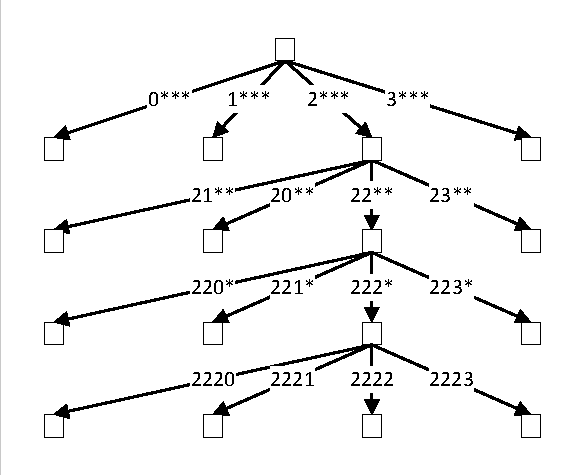
\includegraphics[width=\textwidth]{前缀树.pdf}
%     \caption{page cache的前缀树}
%     \label{fig:前缀树}
% \end{figure}

% 图片\ref{fig:前缀树}展示了page cache的前缀树结构,使用地址的中的几位作为索引,然后在最底层就是具体数据。 最底层每个节点表示一个文件的偏移,值是struct page的指针。但是我们可以复用后面2位,来存储标志位,Linux内核中也已经规定了,所以我们可以复用。



% \begin{table}[h]
%     \centering
%     \caption{标志位}
%     \label{tab:标志位}
%     \begin{tabular}{cc}
%         \toprule
%         \textbf{标志位} & \textbf{说明} \\
%         \midrule
%         00 & data pointer\\
%         \midrule
%         01 & internal entry\\
%         \midrule
%         10 & exceptional entry\\
%         \midrule
%         11 & this bit combination is currently unused/reserved\\
%         \bottomrule
%     \end{tabular}
% \end{table}

% 其中,我们使用文件页中的异常条目没有被使用,所以我们可以复用。

% \begin{figure}[h]
%     \centering
%     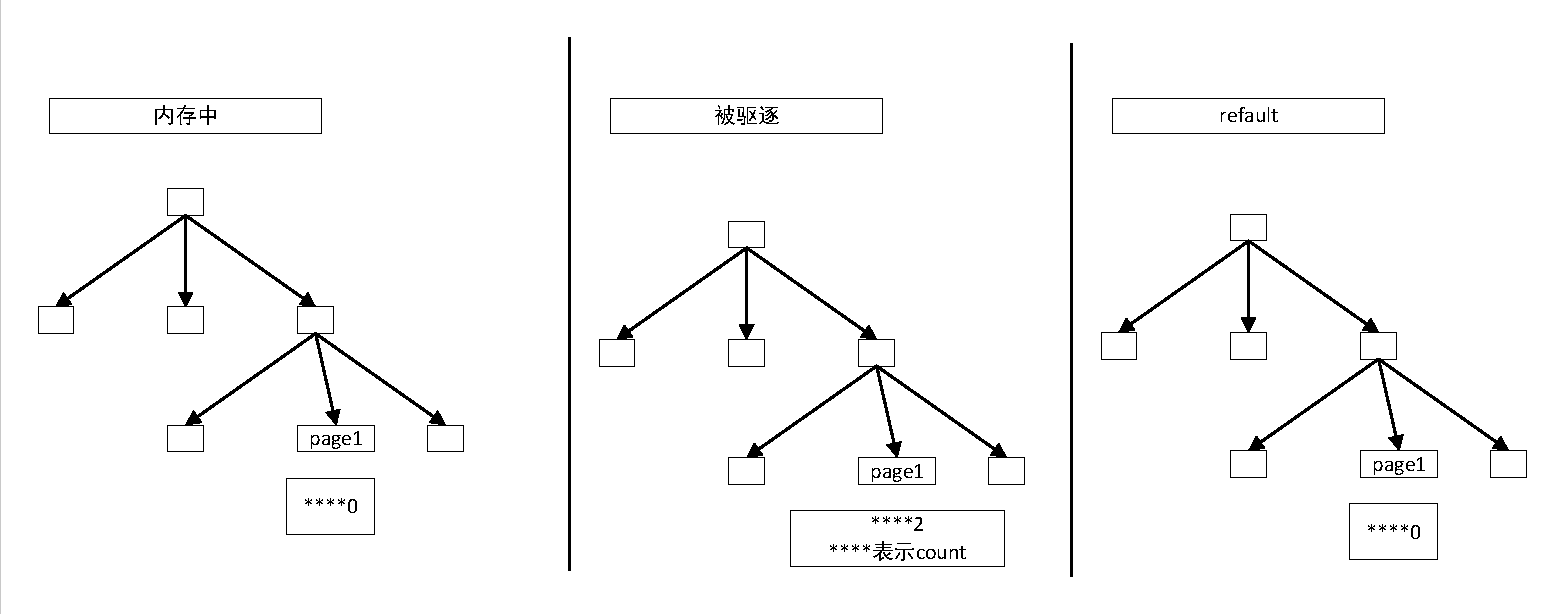
\includegraphics[width=\textwidth]{复用.pdf}
%     \caption{复用}
%     \label{fig:复用}
% \end{figure}

% 图片\ref{fig:复用}展示了复用的情况,当页面的在内存的时候,使用00表示指针,当页面被驱逐的时候,使用10表示异常条目。这种情况既不会导致错误的访问,也可以实现每个页面的计数,也需要需要大量的内存来管理。

% \subsubsection{Shrinker机制的工作原理}

% 由于我们复用了page cache中的条目,导致这部分条目不会被释放,所以需要使用Shrinker机制来释放。
% Linux内核中的Shrinker机制是内存回收子系统的重要组成部分,用于在系统内存压力增大时回收可释放的缓存对象。当系统内存不足时,页面回收进程会调用注册的shrinker回调函数来释放缓存,从而缓解内存压力。Shrinker机制主要应用于各类缓存系统,如inode缓存、dentry缓存和各种文件系统的专用缓存等。

% Shrinker机制在内核的页面回收路径中起作用,特别是在以下场景:
% \begin{itemize}
%     \item 直接内存回收(Direct Reclaim):当分配内存失败且允许等待时触发
%     \item kswapd内核线程:周期性检查内存状态,在内存压力大时主动回收
%     \item 内存紧急回收(Memory Cgroup Reclaim):当某个内存控制组超出限制时触发
% \end{itemize}

% \paragraph {核心数据结构分析}

% Shrinker机制主要涉及两个关键数据结构:\texttt{struct shrinker}和\texttt{struct shrink\_control}。

% \paragraph{shrink\_control结构体}

% \texttt{struct shrink\_control}用于在页面回收子系统和shrinker回调函数之间传递信息。\ref{tab:shrink_control_struct}详细说明了结构体的成员。

% \begin{table}[h]
% \label{tab:shrink_control_struct}
% \centering
% \begin{tabular}{ccc}
% \toprule
% \textbf{成员} & \textbf{类型} & \textbf{说明} \\
% \midrule
% gfp\_mask & gfp\_t & 当前内存分配的标志,指示分配的约束条件 \\
% \midrule
% nid & int & 当前正在进行内存回收的NUMA节点ID \\
% \midrule
% nr\_to\_scan & unsigned long & 指示scan\_objects应尝试回收的对象数量\\
% \midrule
% nr\_scanned & unsigned long & scan\_objects实际处理的对象数量,默认值为nr\_to\_scan \\
% \midrule
% memcg & struct mem\_cgroup * & 当前正在进行内存回收的memory cgroup \\
% \bottomrule
% \end{tabular}
% \caption{shrink\_control结构体成员说明}
% \end{table}

% \paragraph{shrinker结构体}

% \texttt{struct shrinker}定义了一个可注册的回调函数组,用于对可回收缓存施加压力。\ref{tab:shrinker_struct}详细说明了结构体的成员。

% \begin{table}[htbp]
% \label{tab:shrinker_struct}
% \centering
% \begin{tabular}{ccc}
% \toprule
% \textbf{成员} & \textbf{类型} & \textbf{说明} \\
% \midrule
% count\_objects & 函数指针 & 返回缓存中可释放对象的数量,若无可释放对象则返回SHRINK\_EMPTY,若无法确定或应跳过则返回0 \\
% \midrule
% scan\_objects & 函数指针 & 扫描缓存并尝试释放项目,返回已释放对象数量,若因潜在死锁无法继续则返回SHRINK\_STOP \\
% \midrule
% batch & long & 回收批次大小,0表示使用默认值 \\
% \midrule
% seeks & int & 重新创建一个对象所需的磁盘寻道次数,影响回收优先级 \\
% \midrule
% flags & unsigned & shrinker能力标志,如NUMA感知、memcg感知等 \\
% \midrule
% list & struct list\_head & 内部使用,用于将shrinker链接到全局列表 \\
% \midrule
% id & int & 在memcg\_kmem配置下使用的shrinker标识符 \\
% \midrule
% nr\_deferred & atomic\_long\_t * & 按节点统计的待删除对象,用于延迟处理 \\
% \bottomrule
% \end{tabular}
% \caption{shrinker结构体成员说明}
% \end{table}

% \paragraph{Shrinker的注册与使用}

% 内核提供了以下API用于注册和管理shrinker:

% \begin{itemize}
%     \item \texttt{prealloc\_shrinker()}:预分配shrinker相关资源
%     \item \texttt{register\_shrinker\_prepared()}:注册已预分配资源的shrinker
%     \item \texttt{register\_shrinker()}:注册新的shrinker
%     \item \texttt{unregister\_shrinker()}:注销已注册的shrinker
%     \item \texttt{free\_prealloced\_shrinker()}:释放预分配的shrinker资源
% \end{itemize}

% \paragraph{自定义Shrinker的实现方法}

% 要实现一个自定义的shrinker,需要完成以下步骤:

% 1. 定义shrinker结构体并实现必要的回调函数
% 2. 注册shrinker到内核
% 3. 在不再需要时注销shrinker

% Linux内核中的Shrinker机制为各类缓存系统提供了统一的内存回收接口,是内核内存管理的重要组成部分。通过实现count\_objects和scan\_objects回调函数,各子系统可以向内存回收子系统提供可回收对象的信息,并在内存压力下主动释放这些对象。这种机制既保证了内核在内存紧张时的稳定性,又保持了各缓存系统的独立性和灵活性。

\subsection{冷热页面优化的实现原理与机制}

前文的算法设计(\ref{sec:冷热页面优化})提出了基于重用距离(Reuse Distance)来优化冷热页面的思路。为在内核中落地该算法,需要在多个方面进行配合:首先是全局驱逐(eviction)和提升(activation)次数等计数的维护,其次是单个文件页面被驱逐时刻的计数存储,最后还需借助 Shrinker 机制回收不再使用的异常条目,从而保持系统稳定性。下面从整体到局部进行说明。

\subsection{核心计数数据与整体框架}

根据算法需求,我们至少需维护四类计数信息:
\begin{enumerate}
  \item 全局的驱逐和提升次数之和(后文以 \(\mathrm{nr\_count}\) 表示)。
  \item 上次重新故障(refault)统计的次数之和(\(\mathrm{nr\_refault\_last}\))。
  \item 当前时刻累积的重新故障次数之和(\(\mathrm{nr\_refault}\))。
  \item 文件页面被驱逐时对应的驱逐与提升次数之和(记录在页面自身或其关联结构中)。
\end{enumerate}

其中,前 3 项可直接存储在 \texttt{lruvec} 结构体的原子变量中,一旦页面产生驱逐或提升事件,即对 \(\mathrm{nr\_count}\) 执行原子加一。在页面再次加载时,如果满足
\[
  \mathrm{count}(t_2) \;-\; \mathrm{count}(t_1)
  \;\le\;
  L_{\mathrm{active}},
\]
则说明页面在被驱逐后并未经历太长时间就再次被访问,可视为一次重新故障(refault),并相应地增加 \(\mathrm{nr\_refault}\) 计数。

然而,第 4 项对“每个文件页面被驱逐时的计数值”提出了额外要求:需要在页与文件偏移关联的 \texttt{page cache} 中进行记录,且在页面再次载入时还能恢复该计数用于比较。下文详述了如何在 \texttt{page cache} 的前缀树中复用现有结构完成此操作。

\begin{table}[htbp]
  \centering
  \caption{\texttt{lruvec} 结构体中新增的核心成员}
  \label{tab:lruvec_struct}
  \begin{tabular}{ccc}
    \toprule
    \textbf{成员} & \textbf{类型} & \textbf{说明} \\
    \midrule
    \(\mathrm{nr\_count}\) & \texttt{atomic\_long\_t} & 全局驱逐次数与提升次数之和 \\
    \midrule
    \(\mathrm{nr\_refault\_last}\) & \texttt{atomic\_long\_t} & 上次统计时的 refault 次数之和 \\
    \midrule
    \(\mathrm{nr\_refault}\) & \texttt{atomic\_long\_t} & 当前 refault 次数之和 \\
    \bottomrule
  \end{tabular}
\end{table}

\subsubsection{基于异常条目的重用距离记录}

\paragraph{前缀树与异常条目的复用}

Linux 内核中 \texttt{page cache} 的索引结构通常使用前缀树(Radix Tree),底层将文件偏移映射到 \texttt{struct page} 指针。图\ref{fig:前缀树}展示了page cache的前缀树结构,其中每个节点表示一个文件的偏移,值是struct page的指针。

为了实现“页面被驱逐时记下全局计数”的需求,我们复用该指针槽的标志位。  
由于 \texttt{struct page} 对齐方式通常为 16 字节,其指针低位保留 2 位作为标识(\texttt{00}, \texttt{01}, \texttt{10}, \texttt{11}),内核已定义了相应宏来区分“正常指针”、“内部节点”以及“异常条目”等。下表与图示展示了此机制。

\begin{table}[htbp]
  \centering
  \caption{标志位含义与用途}
  \label{tab:标志位}
  \begin{tabular}{cc}
    \toprule
    \textbf{标志位} & \textbf{说明} \\
    \midrule
    \texttt{00} & 指向 \texttt{struct page} 的正常指针 \\
    \texttt{01} & 内部节点 \\
    \texttt{10} & 异常条目(exceptional entry) \\
    \texttt{11} & 目前保留未用 \\
    \bottomrule
  \end{tabular}
\end{table}

\begin{figure}[htbp]
  \centering
  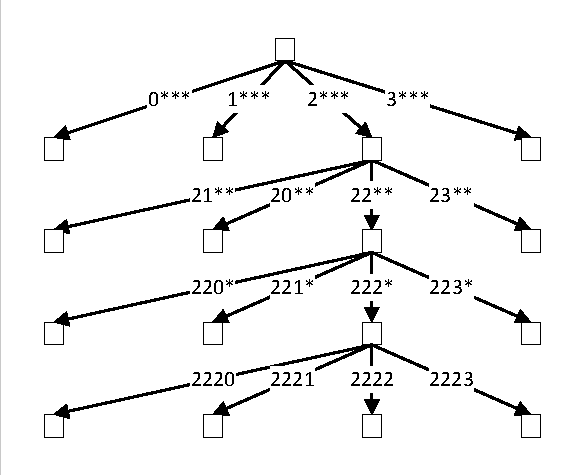
\includegraphics[width=\textwidth]{前缀树.pdf}
  \caption{\texttt{page cache} 的前缀树结构示意}
  \label{fig:前缀树}
\end{figure}

\paragraph{驱逐与再加载时的数据流转}
当某文件页面即将被驱逐(在 \texttt{\_\_remove\_mapping} 中):
\begin{enumerate}
  \item 读取当前 \(\mathrm{nr\_count}\) 原子计数,并将其左移 2 位(为标志位留出空间)。
  \item 与 \(\texttt{10}\) 做或运算,生成“异常条目”,写回前缀树对应索引槽。
  \item 对全局 \(\mathrm{nr\_count}\) 加一,表示发生了一次新的驱逐事件。
  \item 从系统的活动或非活动链表中正式移除该页面,完成驱逐。
\end{enumerate}

当后续对同一文件偏移发生缺页中断(page fault)而需要载入页面时:
\begin{enumerate}
  \item 内核检测到该索引槽存储的标识位并非 \texttt{00}(正常指针),判断其为异常条目。
  \item 提取异常条目中的数值并右移 2 位得到页面被驱逐时的 \(\mathrm{nr\_count}\)。
  \item 计算 \(\mathrm{nr\_count}(t_2) - \mathrm{nr\_count}(t_1)\),若结果不超过活动链表长度 \(L_{\mathrm{active}}\),则视为短期内再访问,此时提升该页面至活动链表,并增大 \(\mathrm{nr\_refault}\) 计数。
  \item 若超出阈值,则仅将该页面放入非活动链表观察,无需更新 \(\mathrm{nr\_refault}\)。
\end{enumerate}

\begin{figure}[htbp]
  \centering
  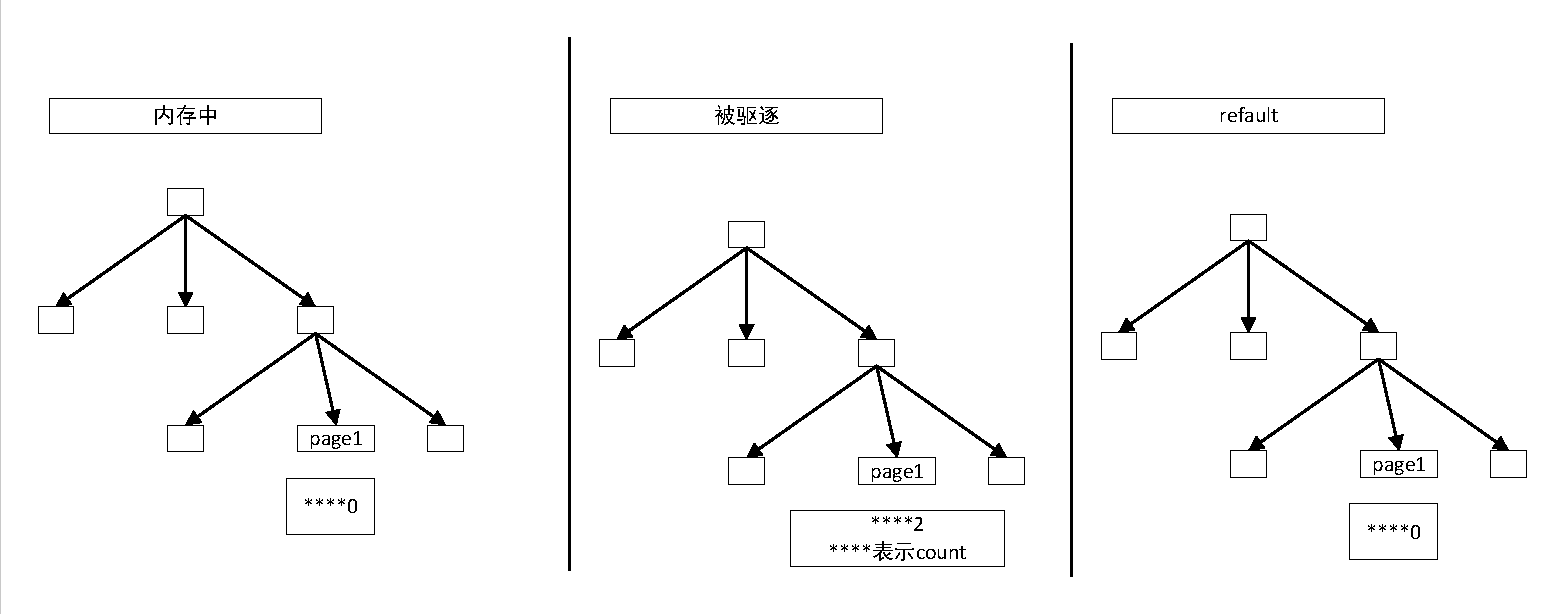
\includegraphics[width=\textwidth]{复用.pdf}
  \caption{利用异常条目存储驱逐时的 \(\mathrm{nr\_count}\)}
  \label{fig:复用}
\end{figure}

如图 \ref{fig:复用} 所示,页面在内存中时使用普通指针(标志位 \texttt{00});被驱逐后则切换为异常条目(标志位 \texttt{10});再加载时可根据此信息计算重用距离并作相应处理。该方法避免了在 \texttt{struct page} 内部额外存储驱逐计数,最大化复用内核已有数据结构。

\subsubsection{Shrinker 机制:缓存回收与资源释放}

\paragraph{为什么需要 Shrinker}

将驱逐过的页面“异常条目”保留在 \texttt{page cache} 的前缀树中,会导致索引节点数量不断累积,若不加以限制,可能造成内存浪费。此时就需要 Shrinker 机制在内存紧张时主动清理这些不再需要的异常条目。

\paragraph{Shrinker 机制概览}

Shrinker 是 Linux 内核内存回收子系统(MM Subsystem)中的统一回调接口,用于管理诸如 inode、dentry 以及各种自定义缓存。内核在以下场景可能触发 Shrinker:
\begin{itemize}
  \item \textbf{直接内存回收(Direct Reclaim)}:进程分配内存失败后尝试同步回收。
  \item \textbf{后台回收线程(kswapd)}:周期性检查系统内存使用情况,在紧张时主动回收。
  \item \textbf{Memory Cgroup 回收(Memcg Reclaim)}:当某内存控制组超出其配额时触发。
\end{itemize}
Shrinker 通过 \texttt{struct shrink\_control}(表 \ref{tab:shrink_control_struct})与 \texttt{struct shrinker}(表 \ref{tab:shrinker_struct})两个核心数据结构向回收框架注册接口,内核则在内存压力情形下调用对应的回调函数执行清理动作。

\begin{table}[htbp]
  \centering
  \caption{\texttt{shrink\_control} 结构体主要字段说明}
  \label{tab:shrink_control_struct}
  \begin{tabular}{ccc}
    \toprule
    \textbf{成员} & \textbf{类型} & \textbf{说明} \\
    \midrule
    \texttt{gfp\_mask} & \texttt{gfp\_t} & 本次内存分配的掩码,指示约束条件 \\
    \texttt{nid} & \texttt{int} & 所在的 NUMA 节点 \\
    \texttt{nr\_to\_scan} & \texttt{unsigned long} & 期望本轮扫描并回收的对象数 \\
    \texttt{nr\_scanned} & \texttt{unsigned long} & 实际扫描对象数量 \\
    \texttt{memcg} & \texttt{struct mem\_cgroup *} & 针对特定 \texttt{memcg} 的回收(若有) \\
    \bottomrule
  \end{tabular}
\end{table}

\begin{table}[htbp]
  \centering
  \caption{\texttt{struct shrinker} 结构体主要字段说明}
  \label{tab:shrinker_struct}
  \begin{tabular}{ccc}
    \toprule
    \textbf{成员} & \textbf{类型} & \textbf{说明} \\
    \midrule
    \texttt{count\_objects} & 函数指针 & 返回可回收对象数,若无可回收则 \texttt{SHRINK\_EMPTY} \\
    \texttt{scan\_objects} & 函数指针 & 实际扫描并回收对象,返回已释放数量 \\
    \texttt{batch} & \texttt{long} & 每次回收的批次大小,默认为 0(使用默认值) \\
    \texttt{seeks} & \texttt{int} & 反映对象重建开销,影响回收优先级 \\
    \texttt{flags} & \texttt{unsigned} & Shrinker 能力标志(NUMA 感知等) \\
    \texttt{list} & \texttt{struct list\_head} & 内核内部使用,用于将 shrinker 链接到全局列表 \\
    \texttt{id} & \texttt{int} & 在 memcg 上下文中的 shrinker 标识 \\
    \texttt{nr\_deferred} & \texttt{atomic\_long\_t *} & 延迟对象数计数 \\
    \bottomrule
  \end{tabular}
\end{table}

\paragraph{自定义 Shrinker 回调的编写}

为释放不再使用的异常条目,需要:
\begin{enumerate}
  \item \textbf{定义 \texttt{struct shrinker} 结构},实现
  \begin{itemize}
    \item \texttt{count\_objects}:返回“可释放异常条目”数量。
    \item \texttt{scan\_objects}:对前缀树节点执行实际回收操作,将长时间未使用的异常条目清理掉。
  \end{itemize}
  \item \textbf{注册 \texttt{shrinker}}:通过 \texttt{register\_shrinker()} 或相关接口将其加入内核回收体系。
  \item \textbf{在不需要时注销 \texttt{shrinker}}:如模块卸载或场景切换时,调用 \texttt{unregister\_shrinker()}。
\end{enumerate}

Shrinker 回调需结合系统内存状态、访问统计等信息,以避免在正常负载时盲目回收、增加额外开销。同时,需确保不会在回收函数中发生较大锁争用或再次触发内存分配,避免死锁等问题。

\subsubsection{总结与展望}

综上所述,本节介绍了冷热页面优化在内核中的具体实现路径:利用 \texttt{lruvec} 中的全局计数器统计驱逐/提升事件,借助异常条目在 \texttt{page cache} 中为每个文件页记录被驱逐时刻的计数值,并通过 Shrinker 机制定期回收冗余异常条目,从而在系统层面有效识别并保留热页面、及时回收冷页面。  
该方法无需额外扩展 \texttt{struct page} 结构即可实现重用距离的近似估算,对大规模服务器和高负载环境具备良好的可扩展性。未来工作可结合多 NUMA 节点访问模式,或针对匿名页面与文件页面配置差异化的回收策略,以进一步提升内存管理的整体效率与性能。
